\documentclass[tikz]{standalone}

\usepackage{newtxtext,newtxmath}

%!TEX root = main.tex

% mytikzset
\usepackage{tikz}
\usetikzlibrary{positioning,arrows,shapes,patterns}
\usetikzlibrary{decorations.pathmorphing}
\usetikzlibrary{decorations.markings}
\usetikzlibrary{decorations.pathreplacing}
\usetikzlibrary{calc}
\usetikzlibrary{patterns}
\usetikzlibrary{decorations.markings}
\usetikzlibrary{petri}

\tikzset{
  vector/.style={thick,double,draw=black, postaction={decorate},
    decoration={markings,mark=at position .6 with {\arrow[black,scale=0.4]{triangle 45}}}},
  axial/.style={thick,double,densely dashed,draw=black, postaction={decorate},
    decoration={markings,mark=at position .6 with {\arrow[black,scale=0.4]{triangle 45}}}},
  gluon/.style={decorate, draw=black,
    decoration={coil,aspect=0.3,segment length=5pt,amplitude=3pt}},
  pseudo/.style={thick, dashed, draw=black, postaction={decorate},
    decoration={markings,mark=at position .6 with {\arrow[red,scale=0.5]{triangle 45}}}},
  scalar/.style={thick,draw=black, postaction={decorate},
    decoration={markings,mark=at position .6 with {\arrow[black,scale=0.5]{triangle 45}}}},
  cut/.style={draw=black, decorate, decoration={snake, segment length=1mm, amplitude=0.2mm}}
}

\definecolor{myGreen}{RGB}{0,127,0}

\definecolor{myGreen}{RGB}{0,127,0}
\definecolor{myViolet}{RGB}{127,0,127}

\begin{document}
\nopagecolor
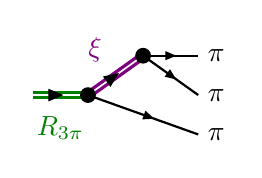
\begin{tikzpicture}[node distance=0.5cm and 0.7cm,baseline=0.cm]
  \coordinate[] (b12);
  \coordinate[right=of b12] (b2);
  \coordinate[above right=of b2] (b13);
  \coordinate[below right=of b13,label=right:$\pi$] (b3);
  \coordinate[right=of b13,label=right:$\pi$] (b4);
  \coordinate[right=of b2] (b25);
  \coordinate[below right=of b25,label=right:$\pi$] (b5);
  \draw[vector,very thick,myGreen]
  (b12) --node[label={below}:{\color{myGreen}$R_{3\pi}$}] {} (b2);
  \draw[scalar]  (b13) -- (b3);
  \draw[vector,very thick,myViolet]
  (b2) -- node[label={above left, xshift=1mm, yshift=-1mm}:{$\xi$}] {} (b13);
  \draw[scalar]  (b2) -- (b5);
  \draw[scalar]  (b13) -- (b4);
  \fill[black]  (b2) circle [radius=0.1];
  \fill[black] (b13) circle [radius=0.1];
\end{tikzpicture}
\end{document}
